277. \begin{center}
\begin{figure}[ht!]
\center{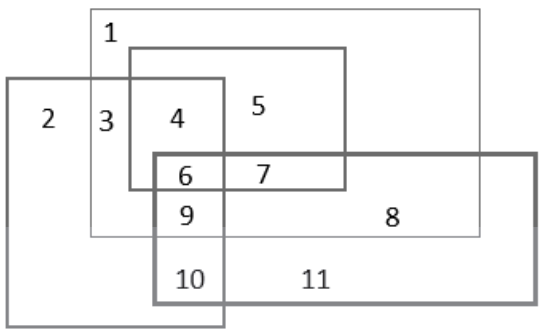
\includegraphics[scale=0.35]{pol.png}}
\end{figure}
\end{center}
На полу лежат четыре прямоугольных ковра, перекрывая друг друга. Напишите номера всех областей, которые покрыты ровно тремя из них.\newpage\noindent
